\documentclass[11pt]{article}
\usepackage[margin=1in, head=1in]{geometry}
\usepackage{amsmath, amssymb, amsthm}
\usepackage{fancyhdr}
\usepackage{graphicx}
\usepackage{pgfplots}

%\usepackage{pdfsync}
\addtolength{\textwidth}{.5in}
\addtolength{\leftmargin}{-1in}
\addtolength{\textheight}{.5in}
\addtolength{\topmargin}{-0.5in}

%\pagestyle{fancy}
%\lhead{MATH 200X }
%\chead{Fall 2007}
%\rhead{FINAL EXAM}
%\lfoot{}
%\cfoot{\thepage}
%\rfoot{}

\setcounter{secnumdepth}{0}
\newcommand{\R}{\mathbb{R}}
\newcommand{\N}{\mathbb{N}}
\newcommand{\Z}{\mathbb{Z}}
\newcommand{\clm}{\par\textit{Claim:}\par}
\newcommand{\diam}{\mathrm{diam}}
\newcommand{\sect}{\textsection}

\parindent=0in
\parskip=0.5\baselineskip

\begin{document}
\newgeometry{top=3in}
\begin{center}
\vspace{2in}

\huge{Math 156 PRECALCULUS \\
Fall 2015}

\vfill

\huge{\bf{Quiz 3 -- Version One}}\\

\vspace{0.5in}

\large{Thursday, September 24, 2015}\\

\vfill


{\huge{Name:{\underline{\hspace{2in}}}}}
\vfill
This quiz has 8 problems worth a total of 30 points. It is TWO SIDED. 
\vfill
\end{center}
\newpage
\restoregeometry
\begin{enumerate}
%1.8.34
\item (3 points) Solve the linear inequality \scalebox{1.2}{$-3 \leq 4-5x <9$} and express the solutions using interval notation.

\begin{flushright}{Answer: \underline{\hspace{2in}}}\end{flushright}

\vspace{1in}
%1.8.84
    \item (4 points) Solve the absolute value inequality \scalebox{1.2}{$\left\vert {x-5} \right\vert \geq 8$} and express the answer using interval notation.

\begin{flushright}{Answer: \underline{\hspace{2in}}}\end{flushright}
\vspace{1in}
%1.8.51
\item (4 points) Solve the nonlinear inequality \scalebox{1.2}{$(x+2)(x-3) < 0$} and express the solution using interval notation.

\begin{flushright}{Answer: \underline{\hspace{2in}}}\end{flushright}
\vfill
%1.9.27
\item (2 points each) Given the pair of points $(-4,6)$ and $(2,5),$ (a) find the distance between the points and (b) the midpoint of the segment that joins them.

\begin{flushright}{distance: \underline{\hspace{2in}}}\end{flushright}

\begin{flushright}{midpoint: \underline{\hspace{2in}}}\end{flushright}

\vspace{0.25in}
%%%%%%%%%%%%%%% NEW PAGE %%%%%%%%%%
\newpage
% 1.9.87
\item (3 points) Find the center and radius of the circle $(x-1)^2+(x+10)^2=9.$

\begin{flushright}{center: \underline{\hspace{2in}}}\end{flushright}

\begin{flushright}{radius: \underline{\hspace{2in}}}\end{flushright}

% 1.10.32
\item (4 points) Find an equation of the line through the points $(-2,6)$ and $(4,5).$

\begin{flushright}{Answer: \underline{\hspace{2in}}}\end{flushright}
\vfill

%1.10.47
\item (4 points) Find an equation of the line through the point $(1,2)$ perpendicular to the line $y=3x+2.$

\begin{flushright}{Answer: \underline{\hspace{2in}}}\end{flushright}
\vfill

%1.11.38
\item (4 points) Use the graphs below to solve the inequality $3x+10 \leq 6x^2-x^3.$\\
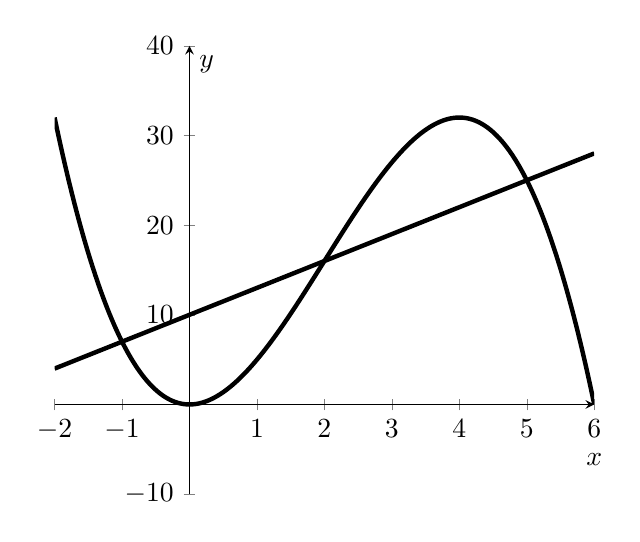
\begin{tikzpicture}[scale=1]
\begin{axis}[
        axis x line=middle, 
        axis y line=middle, 
        ymax=40, 
        ymin=-10,
        ylabel=$y$, 
        xtick={-2,-1,1,2,3,4,5,6},
        x label style={at={(current axis.right of origin)},anchor=north, below=5mm},
         xlabel=$x$,
        %x label style={at={(axis description cs:4,-1)},anchor=north},
        ]
    \addplot[domain=-2:6, samples=400, black, ultra thick]  {3*x+10};
    \addplot[domain=-2:6, samples=400, black, ultra thick]  {6*x^2-x^3};
\end{axis}
\end{tikzpicture}
\begin{flushright}{Answer: \underline{\hspace{2in}}}\end{flushright}

\end{enumerate}
\end{document}